\documentclass[a4paper,12pt]{article}

\usepackage [utf8x] {inputenc} %кодировка исходного текста
\usepackage [T2A] {fontenc} %кодировка
\usepackage [english, russian] {babel}
\usepackage{color}
\usepackage{amsmath, amsfonts, amssymb, amsthm, mathtools}
\usepackage{graphicx}
\graphicspath{{.}}
\DeclareGraphicsExtensions{.pdf,.png,.jpg}
\righthyphenmin=2


\title{Лабораторная работа 1}
\author{Калашников Михаил, Б03-205}
\date{}


\begin{document}

\maketitle{Вставки и переходы}

\begin{enumerate}

\setcounter{enumi}{0}

\item Воспользуемся ассемблерной вставкой и сгенерируем листинги.

\begin{figure}[h!]
  \centering
  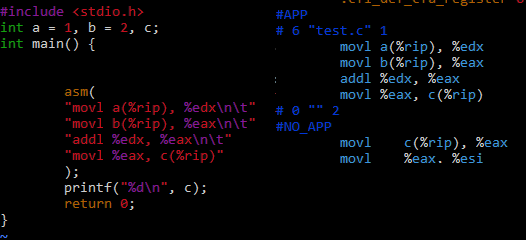
\includegraphics[width=0.8\linewidth]{images/asm1_1.png}
  \caption{К пункту 1}
\end{figure}

\item[2-4.] Вставим в код условный опретор и получим в листинге метку, команду перехода и оператор сравнения. Также воссоздадим условный оператор с помощью листинга, пользуясь метками куст и лампа (не спрашивай).
\begin{figure}[h!]
  \centering
  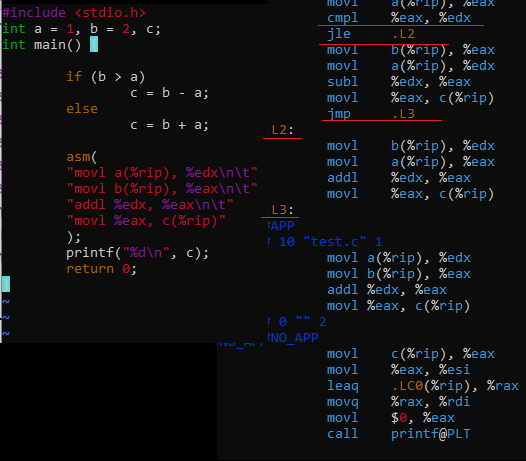
\includegraphics[width=0.6\linewidth]{images/asm1_2.png}
  \caption{К пунктам 2-4}
\end{figure}

\begin{figure}[h!]
  \centering
  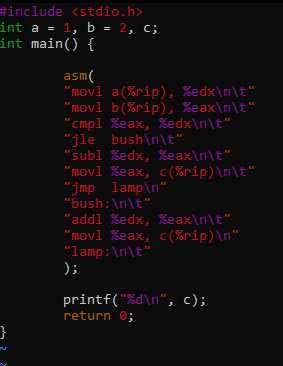
\includegraphics[width=0.6\linewidth]{images/asm1_3.png}
  \caption{К пунктам 2-4}
\end{figure}

\setcounter{enumi}{4}

\item Создадим статический одномерный массив. В объявлении выделится 4 * 10 (размер массива) байт. Обращение происходит с помощью команды lea. Инициализация двумерных массивов аналогична.

\begin{figure}[h!]
  \centering
  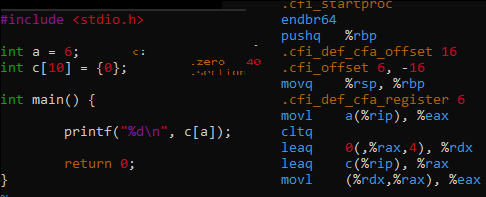
\includegraphics[width=0.6\linewidth]{images/asm1_4.png}
  \caption{К пункту 5}
\end{figure}

\item Очевидно, безусловные команды перехода (jmp) осуществляют безусловный переход, а условные (e.g., je) -- при удовлетворении некоего условия (предыдущей команды cmp). Проверить их работу мы сможем в следующем пункте.

\item Условный оператор уже был организован в предыдущих пунктах. Реализуем цикл for. Он должен десять раз инкрементировать переменную 1. Он действительно работает как и представлено на картинке. Остальные виды циклов реализуются очень похожим простым образом.

\begin{figure}[h!]
  \centering
  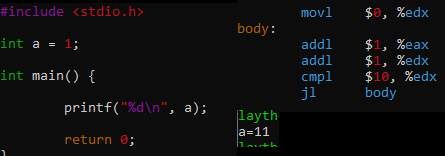
\includegraphics[width=0.6\linewidth]{images/asm1_5.png}
  \caption{К пункту 7}
\end{figure}

\item Команда loop сильно упрощает реализацию цикла. Ниже представлен тот же цикл for из прошлого пункта, но с использованием оператора loop.

\begin{figure}[h!]
  \centering
  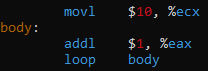
\includegraphics[width=0.6\linewidth]{images/asm1_6.png}
  \caption{К пункту 8}
\end{figure}

\item На картинке представлена реализация поиска максимума из двух чисел.

\begin{figure}[h!]
  \centering
  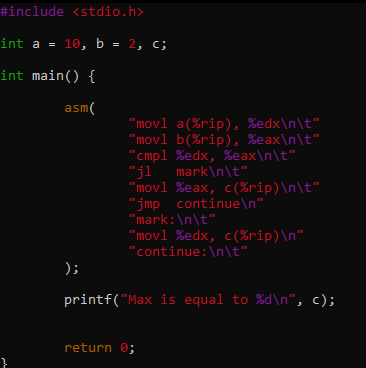
\includegraphics[width=0.6\linewidth]{images/asm1_7.png}
  \caption{К пункту 9}
\end{figure}

\item На картинке представлена реализация поиска суммы элементов массива.

\begin{figure}[h!]
  \centering
  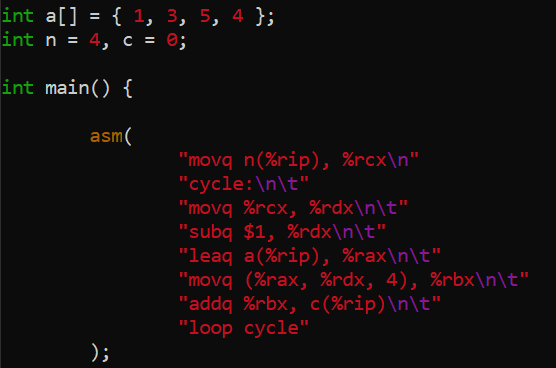
\includegraphics[width=0.6\linewidth]{images/asm1_8.png}
  \caption{К пункту 10}
\end{figure}

\item Теперь реализуем сортировку пузырьком. Вставка приложена к отчету в отдельном файле, графики представлены на картинке. Дефолтная сортировка пузырьком с флагами -O1 и -O2 оказывается быстрее сортировки, написанной целиком на ассемблере.

\begin{figure}[h!]
  \centering
  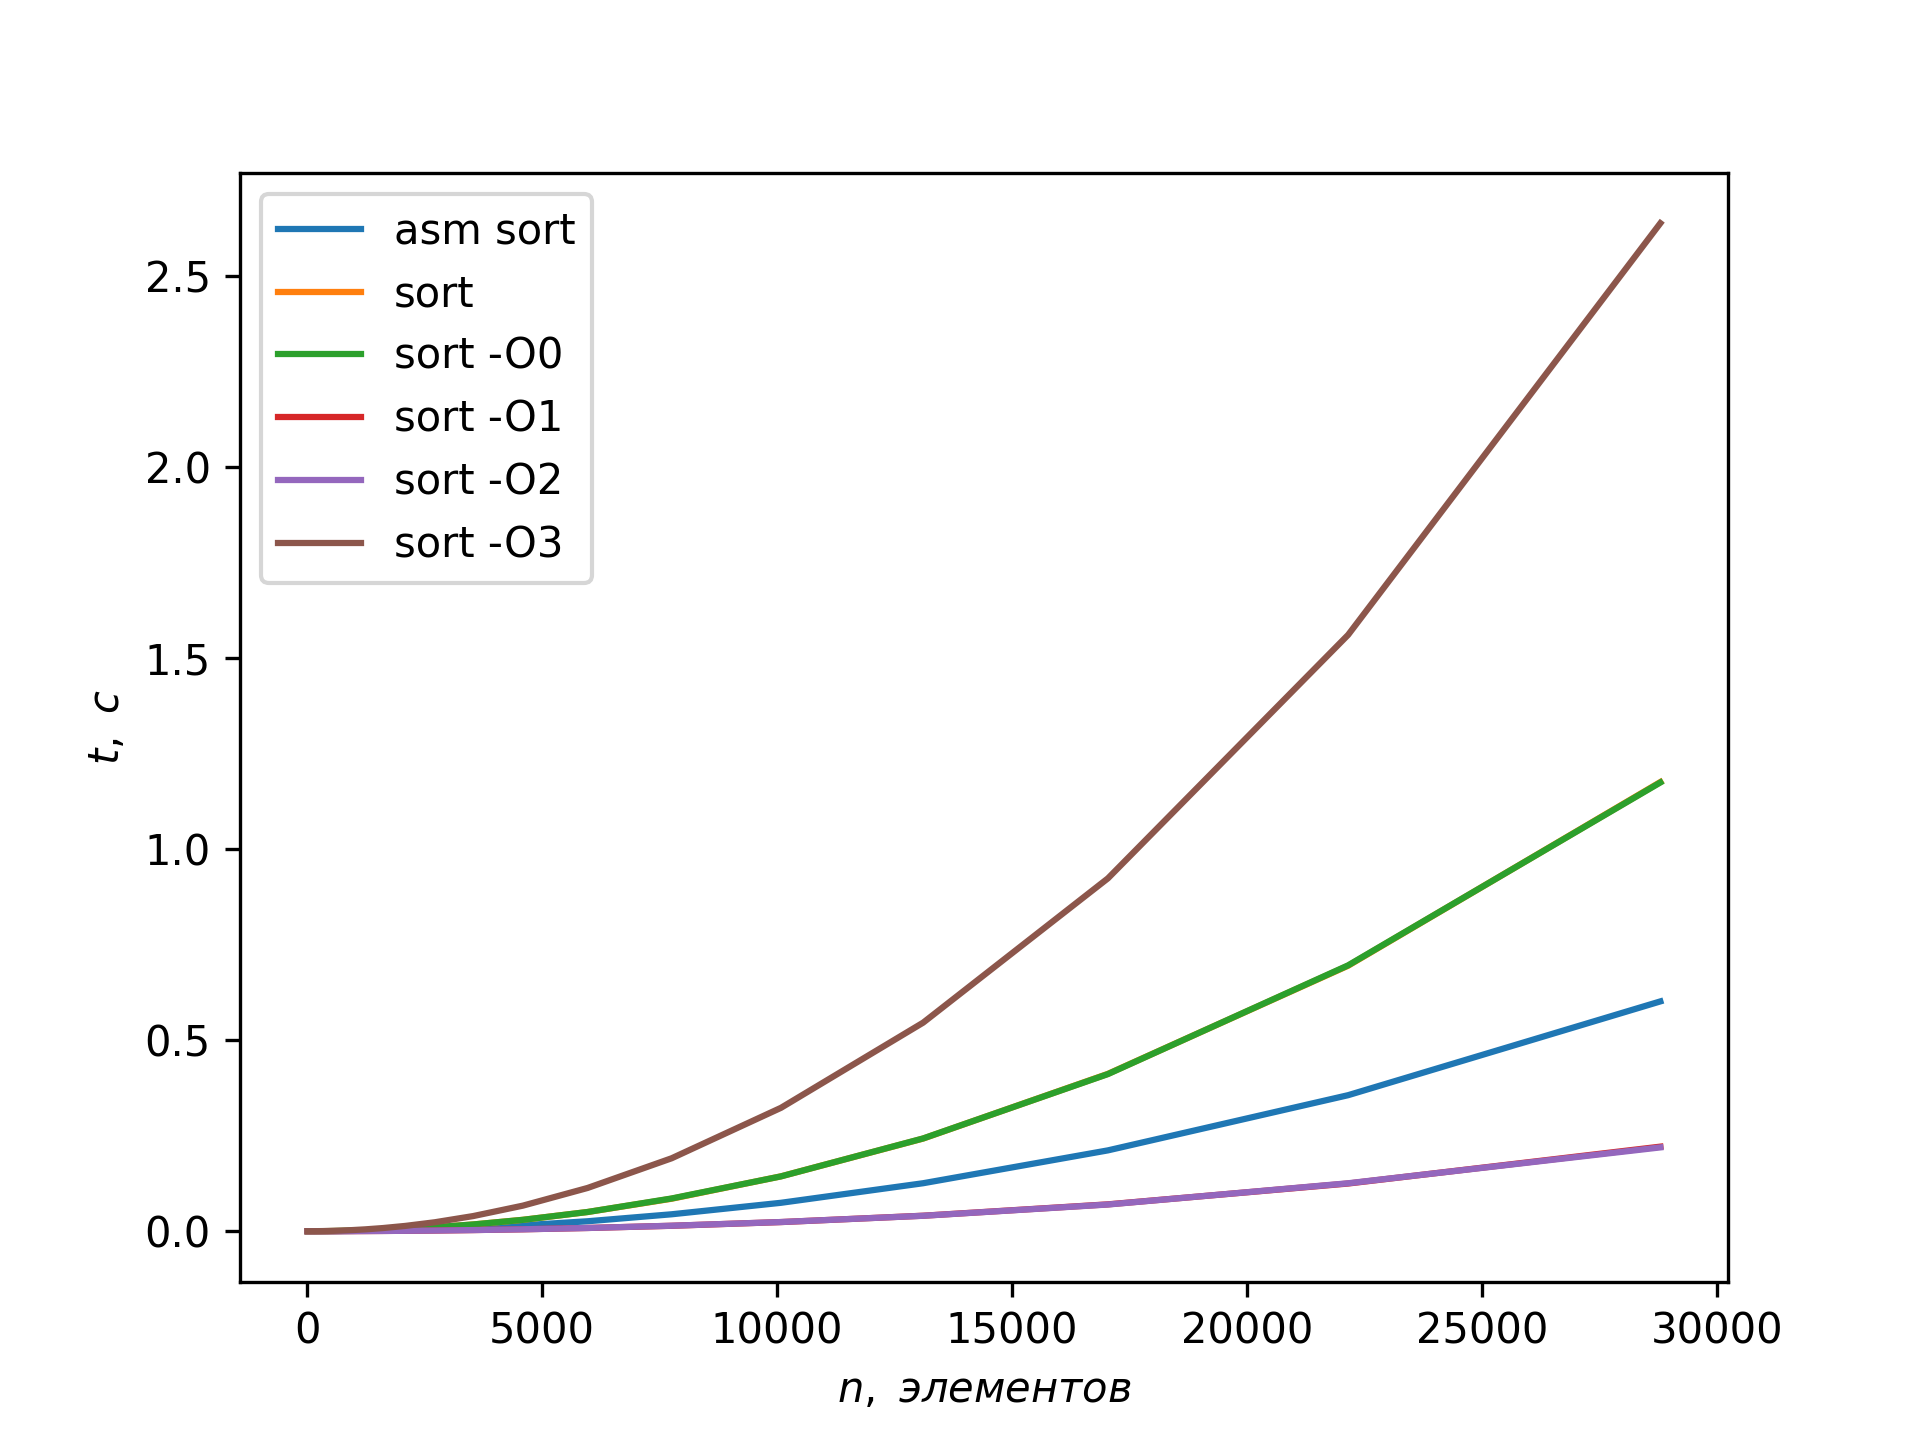
\includegraphics[width=1\linewidth]{images/asm1_0.png}
  \caption{К пункту 11}
\end{figure}


\end{enumerate}

\end{document}